%\documentclass[10pt,a4paper]{article}
\documentclass[11pt,a4paper]{article}
%\documentclass[11pt,a4paper]{article}

%\usepackage[left=1cm, right=1cm, top=1cm, bottom=2cm]{geometry}
\usepackage[left=0.5cm, right=0.5cm, top=0.5cm, bottom=1.5cm]{geometry}
%\usepackage[margin=2cm]{geometry}

\usepackage[utf8]{inputenc}
\usepackage[T1]{fontenc}
\usepackage[french]{babel}
\usepackage{hyperref}
\usepackage{graphicx}
\usepackage{float}
\usepackage{calc}
\usepackage{amssymb}
\usepackage{xcolor}

\begin{document}

	\title{\vspace*{-1.5cm}Dubins and Reeds-Shepp paths\vspace{-0.5cm}}
	\author{Benjamin Loison}
	\date{\vspace*{-0.25cm}January 2022}
	
	\maketitle

	\setlength{\parindent}{0cm}
	
	\vspace*{-0.5cm}
	
	First we will see the Dubins paths, then some implementation details of this type of algorithm, then we will study the Reeds-Shepp paths and the different possible simplifications.
	I will now introduce the Dubins and Reeds-Shepp paths with some examples to start:
	
	\section{Dubins paths}
	
	\begin{minipage}{0.8\textwidth}
	\raggedright
	For example, let's imagine that at the green starting point it is a human being who wants to go to the red ending point, if I ask you what is a shortest way, you will answer me that it is enough to go in a straight line from the green point to the red point.
	\end{minipage}
	\begin{minipage}{0.2\textwidth}
	\includegraphics[width=\linewidth]{Illustrations/humanSummary.png}
	\end{minipage}\\
	
		\begin{minipage}{0.8\textwidth}
	\raggedright
	Okay, but in fact the human being is oriented to the north at the green starting point and we want him to arrive oriented to the east at the red ending point. If I ask you the same question: what is a shortest way between these two oriented positions, assuming that turning around is instantaneous, you will still answer that the problem is trivial and that it is enough to turn at the green starting point towards the red arrival point and then to walk straight to the red arrival point and to orient yourself towards the east.
	\end{minipage}
	\begin{minipage}{0.2\textwidth}
	\includegraphics[width=\linewidth]{Illustrations/humanOrientedSummary.png}
	\end{minipage}\\
	
	\begin{minipage}{0.8\textwidth}
	\raggedright
	Okay, but in fact, let's consider a robot that can only move forward instead of the human being, we stay on the same problem but this time physically we realize that the robot can't turn on itself by staying on the spot.
	That is to say, when we tell the robot to turn to the left at the maximum, we observe a turning radius, of a few meters here. With this constraint of only being able to move forward, or to turn left at the maximum, or to turn right at the maximum, I ask you the same question again: what is a shortest path for this robot between these two oriented positions ?
	\end{minipage}
	\begin{minipage}{0.2\textwidth}
	\includegraphics[width=\linewidth]{Illustrations/robotMinimumCircleSummary.png}
	\end{minipage}\\
	
	\begin{minipage}{0.8\textwidth}
	\raggedright
	Then the problem is no longer trivial in the general case, although on this example, we can see that this is a shortest path. This shortest path treated in the case of the robot is called Dubins path because this problem, to find a shortest path between two oriented positions for a robot that can only go forward or turn left at the maximum or turn right at the maximum with a non-zero turning radius, has been solved by Lester Dubins in 1957.
	\end{minipage}
	\begin{minipage}{0.2\textwidth}
	\includegraphics[width=\linewidth]{Illustrations/002Summary.png}
	\end{minipage}\\
	
	\begin{minipage}{0.9\textwidth}
	\raggedright
	Indeed in the general case where the two oriented positions are arbitrary, he showed that a shorter path was necessarily of the form CSC or CCC. With C meaning "curve" (i.e. turn left or right) and S meaning "straight" (i.e. go straight). Similarly, R stands for "right" and L for "left". Going back to the previous example, the Dubins path found was an LSR i.e. at the beginning the robot turns left, then goes straight then turns right.
	\end{minipage}
	\begin{minipage}{0.1\textwidth}
	\includegraphics[width=\linewidth]{Illustrations/combinaisonsSummary.png}
	\end{minipage}\\
	% could not display the image - doesn't help because on first page
	
	\section{Implementation details}
	
	It is interesting to note that the algorithm of finding a shortest path, using Dubins' approach, has a constant complexity because this algorithm consists in computing the 6 possible paths and determining a shortest.
	
	Although the complexity is constant, as well as for the algorithm that we will see in a few moments, it can be interesting to avoid doing some heavy calculations involving trigonometric functions by using a table of angles that indicate in which bounds and only in these bounds the different paths are optimized.\\
	
	\begin{minipage}{0.8\textwidth}
	\raggedright
	The different points of interest where the behavior of the robot changes, i.e. from turning right to going straight for example, are determined with the inner and outer tangents to the two circles defined by the oriented positions of departure and arrival. Indeed, in the case where the two circles are outside each other, there are generally four distinct lines which are tangent to the two circles. For two of them, the external tangents, here in yellow, the two circles are on the same side of the tangent, for the other two, here in light blue, the internal tangents, the circles are on each side. Once these tangents are drawn, we can quickly find the shortest path obtained. I will not detail how we obtain these tangents but it is done by simple calculations.
	\end{minipage}
	\begin{minipage}{0.2\textwidth}
	\includegraphics[width=\linewidth]{Illustrations/001tangentsSummary.png}
	\end{minipage}\\
	
	Furthermore, once the sequence of movements that the robot must perform is calculated, we can use the following differential equations to obtain the coordinates of the robot at a given time. We can either integrate with the Euler method or we can make a more precise calculation considering the point starting the arc or the segment and calculate where the robot is on this portion of the path. Moreover, if we use the first method, we can make the size of the step $\delta$ depend on the distance of the path to travel.
	% the follwoing
	
	\section{Reeds-Shepp paths}
	
	\begin{minipage}{0.8\textwidth}
	\raggedright
	So if we come back to the initial problem, of a robot looking for a shortest path from an oriented start position to an oriented finish position, restricting the movements of this robot to go straight, turn left and turn right with a non-zero turning radius. If this time we add the possibility for the robot to go backwards all the way, backwards to the left and backwards to the right and I ask you the same question: what is a shortest path, there is enough to make you think.
	Well, here is the answer. The robot will first turn left backwards, then go straight backwards and then turn slightly right backwards. Knowing that obviously a shortest path from Reeds to Shepp is at least as short as a shortest path from Dubins.
	\end{minipage}
	\begin{minipage}{0.2\textwidth}
	\includegraphics[width=\linewidth]{Illustrations/ReedsSheppBeautifulSummary.png}
	\end{minipage}\\
	
		\begin{minipage}{0.8\textwidth}
	\raggedright
	In the paper by J. A. Reeds and L. A. Shepp published in 1990, they solve this problem of the robot also being able to go backwards in the general case. Unlike Dubins' paths where there were only 6 possibilities, Reeds and Shepp's paths have 48 different possibilities. Also here the subscripts indicate the length of the arc or the length of the segment involved and the subscript plus or minus to the power means when it is plus, a forward movement and minus when it is a backward movement. And the vertical bars mean a change in direction. Reeds and Shepp solved this problem using a computer, in fact the computer helped them find this set of possibilities and helped them write a proof that this set is sufficient and Reeds and Shepp facilitated the proof so that it is readable by a human being. Moreover they point out that one can relate the 48 possibilities to 9 possibilities by noticing similarities in the different paths. We will now study these simplifications.
	\end{minipage}
	%\begin{minipage}{0.2\textwidth}
	%\includegraphics[width=\linewidth]{Illustrations/ReedsSheppPossibilitiesNoTitleNoTimeflipNoReflectNoReverseSummary0.png}
	%\end{minipage}
	%\begin{minipage}{0.2\textwidth}
	%\includegraphics[width=\linewidth]{Illustrations/ReedsSheppPossibilitiesNoTitleNoTimeflipNoReflectNoReverseSummary1.png}
	%\end{minipage}
	\begin{minipage}{0.2\textwidth}
	\includegraphics[width=0.84\linewidth]{Illustrations/ReedsSheppPossibilitiesNoTitleNoTimeflipNoReflectNoReverseSummary.png}
	\end{minipage}\\
	
	\begin{minipage}{0.8\textwidth}
	\raggedright
	Indeed, noticing the fact that a path $l^-r^+s^+l^+$ here in dark blue from (0, 0, 0) to ($x, y, \phi$) and that this same path where we change the direction of each subpath thus $l^+r^-s^-l^-$ here in light blue from (0, 0, 0) to ($-x,y,-\phi$). On the drawing I made, this \textcolor{red}{"timeflip"} property is clear.
	\end{minipage}
	\begin{minipage}{0.2\textwidth}
	\raggedright
	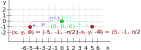
\includegraphics[width=\linewidth]{Illustrations/timeflip.png}
	\end{minipage}\\
	% could precise what inverse mean because it is used several times - seems ok now
	
	\begin{minipage}{0.8\textwidth}
	\raggedright
	In a similar way we can notice the following property: a path $r^+l^-s^-r^-$ from (0, 0, 0) to ($x, y, \phi$) and that this same path reverses the directions, that is to say that the left turns become right turns and vice versa, this path is thus $l^+r^-s^-l^-$ from (0, 0, 0) to ($x,-y,-\phi$). Again, this \textcolor{green}{"reflect"} property is clear from my example.
	\end{minipage}
	\begin{minipage}{0.2\textwidth}
	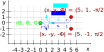
\includegraphics[width=\linewidth]{Illustrations/reflect.png}
	\end{minipage}\\
	
	\begin{minipage}{0.8\textwidth}
	\raggedright
	In a similar way one can notice that by inverting the order of a path, $l^-s^-r^-l^+$, thus obtaining the path $l^+s^+r^+l^-$ the end point is no longer ($x, y, \phi$) but ($x$cos $\phi+y$sin $\phi$, $x$sin $\phi-y$cos $\phi$, $\phi$). A little harder to convince oneself of the truth of this property but in any case on the example, this \textcolor{blue}{"reverse"} property is verified.
	\end{minipage}
	\begin{minipage}{0.2\textwidth}
	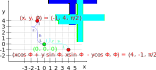
\includegraphics[width=\linewidth]{Illustrations/reverse.png}
	\end{minipage}\\
	
	Moreover, Reeds and Shepp claim that all formulas with two subpossibilities have one too many subpossibilities because they are never observed within an optimal path and that one of the two subpossibilities may therefore not be considered each time. % not so important
	
	To deal with the simplest case of $l_t^+s_u^+l_v^+$ to give you an idea of the trigonometry that is applied in each case. So we have $u$ and $t$ obtained through the inverse of a polar transformation of $x -$ sin $\phi$ and $y - 1 +$ cos $\phi$, we obtain $v$ by postponing $\theta - t$ between 0 and $2\pi$. Moreover, as Reeds and Shepp point out, the path cannot be optimal if $t$ or $v$ is outside of $[0, \pi]$
	% reminding t, u and v is maybe too much here
	% Here the indices $t, u$ and $v$ are used to indicate the length of the arc or the segment considered.
	
	\section{Conclusion}
	
	In practice, the Dubins and Reeds-Shepp paths cannot be used as they are in reality because it is difficult to make a robot follow a calculated path perfectly. In addition to the fact that the Dubins and Reeds-Shepp paths are not very realistic since they do not deal with speed variation, nor with the possibility of not steering to the maximum, nor with the non-perfect adherence of the vehicles in the curves.
	
	Another problem is that these algorithms do not deal with the presence of obstacles, which is unrealistic. However one can use a rapidly-exploring random tree, which consists in searching efficiently in a space by building a random tree that fills the space. Indeed instead of considering the usual distance in $\mathbb{R}^2$ one can use the pseudo distance induced by Dubins paths or even the Reeds-Shepp one which is probably a distance because it is symmetrical since backward movements are allowed.
	
	\section{References}
	
	\begin{itemize}
		\item Optimal paths for a car that goes both forwards and backwards (1990), J. A. Reeds and L. A. Shepp
		\item A Comprehensive, Step-by-Step Tutorial to Computing Dubins' Paths (2013), Andy G's Blog
	\end{itemize}

\end{document}